% \chapter{From encoding to semantics-preserving interactivity}
% \label{chp:ipenrose}

% Diagrams live in the context of surrounding text, overlaid annotations, and human gestures. The web opens up opportunities for even richer in-context interaction. In education, though students spend more time on digital platforms, they often see diagrams that are presented exactly as before: blurry, static, and ornamental. In addition to their values as an external, static representation of knowledge, diagrams are also beneficial when people learn \emph{with}, instead of \emph{from} them~\cite{learningWithRepresentations}.  Prior work shows interacting with visual representations has unique benefits to learning \cite{drawingToLearn, VisualexplanationsImprovesLearning}. In contrast with a static diagram, \textbf{a semantics-preserving interactive diagram allows students to rapidly explore alternatives, understand the underlying rules of a visual representation, and receive instant feedback on their actions.} Meaningful interaction with diagrams helps students move from passive recognition to active synthesis of visual representations~\cite{bloomRevised}.

% Sadly, interactive diagrams are scarce in the wild. Most interactive documents require authors to be proficient in general-purpose programming and have decent knowledge in handling low-level events like mouse down/up, hover, etc. As a result, a simple interactive diagram often takes up 100s of lines-of-code and can be hard to debug~\cite{callbackSpaghetti, usabilityInteractionTools}. Additionally, because interactive diagrams change a lot, authors often need to reason about a collection of diagrams, making the task even harder.

% \Penrose and \Edgeworth elevate the semantics of diagrams from low-level primitives to mathematically meaningful notations. Specifically, \Penrose encodes both the translational semantics of how notations are translated to diagrams, and the visual semantics of how shape primitives relate to each other expressed as constraints. By exploiting both, we can automatically support semantics-preserving interactive diagrams. In this section, I investigate how to build interactive diagram activities that are automatically derived from \Penrose diagrams and easily created without extensive programming efforts. In short, I propose to \textbf{(1) simplify programming interactive diagrams and (2) provide students with rich, automated feedback by leveraging the encoding of visual representations}. 

% \section{Motivating example}
% \label{sec:ipenrose-example}

% Consider the first diagram in a popular explorable explanation piece ''Eigenvectors and Eigenvalues Explained Visually~\footnote{\url{https://setosa.io/ev/eigenvectors-and-eigenvalues/}}.''  The diagram is one of a series of interactive diagrams showing the visual properties of eigenvalues and eigenvectors: it shows a visual interpretation of matrices as linear transformations: matrix $A$ with columns $a_1$ and $a_2$ transforms $v$ to $Av$. In the diagram, $a_1$, $a_2$ and $v$ are all draggable. 

% \begin{figure}[h]
%     \centering
%     \includegraphics[width=0.8\linewidth]{assets/chapter-4/eigen-visually.pdf}
% \end{figure}

% Seeing what varies and what doesn't is an important form of \emph{feedback} that fosters conceptual understanding. The reader gains an initial understanding of how columns of $A$ impact $Av$’s value through interacting with the diagram: dragging any of $a_1$, $a_2$ and $v$ affects the position of $Av$. 

% In the original code repository~\footnote{\url{https://github.com/vicapow/explained-visually/tree/master/client/explanations/eigenvectors-and-eigenvalues}}, the authors wrote about a hundred lines of JavaScript with D3.js to make the first diagram. Although D3.js and Angular already provide significant support, it's still a lot of work to handle mouse down/up/hover events, and to keep track of intermediate values during dragging. 

% To reproduce this diagram in \Penrose, one can write a simple \Substance program in the linear algebra domain~\cite[Section 5.4]{penrose}. 

% \begin{figure}[h]
%     \centering
%     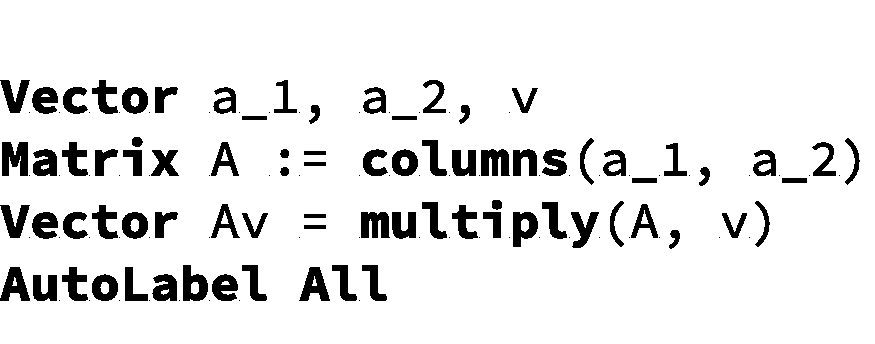
\includegraphics[width=0.4\linewidth]{assets/chapter-4/eigen-substance.pdf}
% \end{figure}

% With the core system, the trio generates a static SVG diagram. Under the hood, every \sub{Vector} is represented visually as an arrow starting at the origin ($a_1$, $a_2$), or a single point ($v$). They are all degrees of freedom (DOF) in the optimization problem. In other words, both the x and y-components of the arrow-end of  $a_1$, $a_2$, and the point representing $v$ are free to move on the canvas. Following the original design of the explorable, the system surfaces the DOFs as draggable points. Whenever the user drags the end of one of the arrows, the optimizer takes the new position as a part of the final solution, and solves the rest of the optimization problem. Effectively, by using this simple and generalizable strategy, which I will discuss in the following sections, the system can reproduce the interactive design using the \Penrose trio for a static diagram \emph{without a single line of code added}.

% \section{Semantics-preserving interactivity as feedback}
% \label{sec:semantic-drag}

% \begin{proposed}
% \cref{sec:ipenrose-example} is an example of a set of interactive behaviors that can be automatically derived from a \Penrose trio without any additional programming.  Specifically, the example leverages how \Penrose encodes visual semantics: \Penrose compiles a program trio to computational and optimization graphs with degrees-of-freedom (DOF)~\cite[Section 4.1.2-3]{penrose}. Degrees-of-freedom determine a diagram instance in \Penrose. They are ``free'' variables within the computational graph and non-constant root nodes in the optimization graph. DOFs are the key to generate a family of diagrams: by manipulating DOFs, the optimizer solves for different diagrams that satisfy the constraint set defined by the trio. In other words, DOFs are a concise representation for interaction. In this section, I use \emph{dragging} as a case study and show a few ways of manipulating the DOFs in a semantics-preserving manner. 

% As a reasonable default, the system can find positional properties in the DOFs and make them draggable. In \cref{sec:ipenrose-example}, the relevant \Style blocks define a simple computational graph for the \Substance program, where \sty{a_1.data}, \sty{a_2 .data}, and \sty{v.data} are DOFs. \cref{fig:eigen-comp-graph} shows the graph for \sty{a_1}’s properties. To accomplish the interactivity in the example, the system can analyze the computational graph to find DOFs and their aliases, \ie, child nodes that are assigned values of the DOFs. For instance, \sty{a_1.data} is a DOF and \sty{a_1.icon.end} references \sty{a_1.data}. In contrast, \sty{Av.end} is not made draggable because it's not a DOF nor an alias in the computational graph: its value is computed by \sty{matmul(a_1.data, a_2.data)}.

% \vspace{10pt}
% \begin{figure}[h]
%     \centering
%     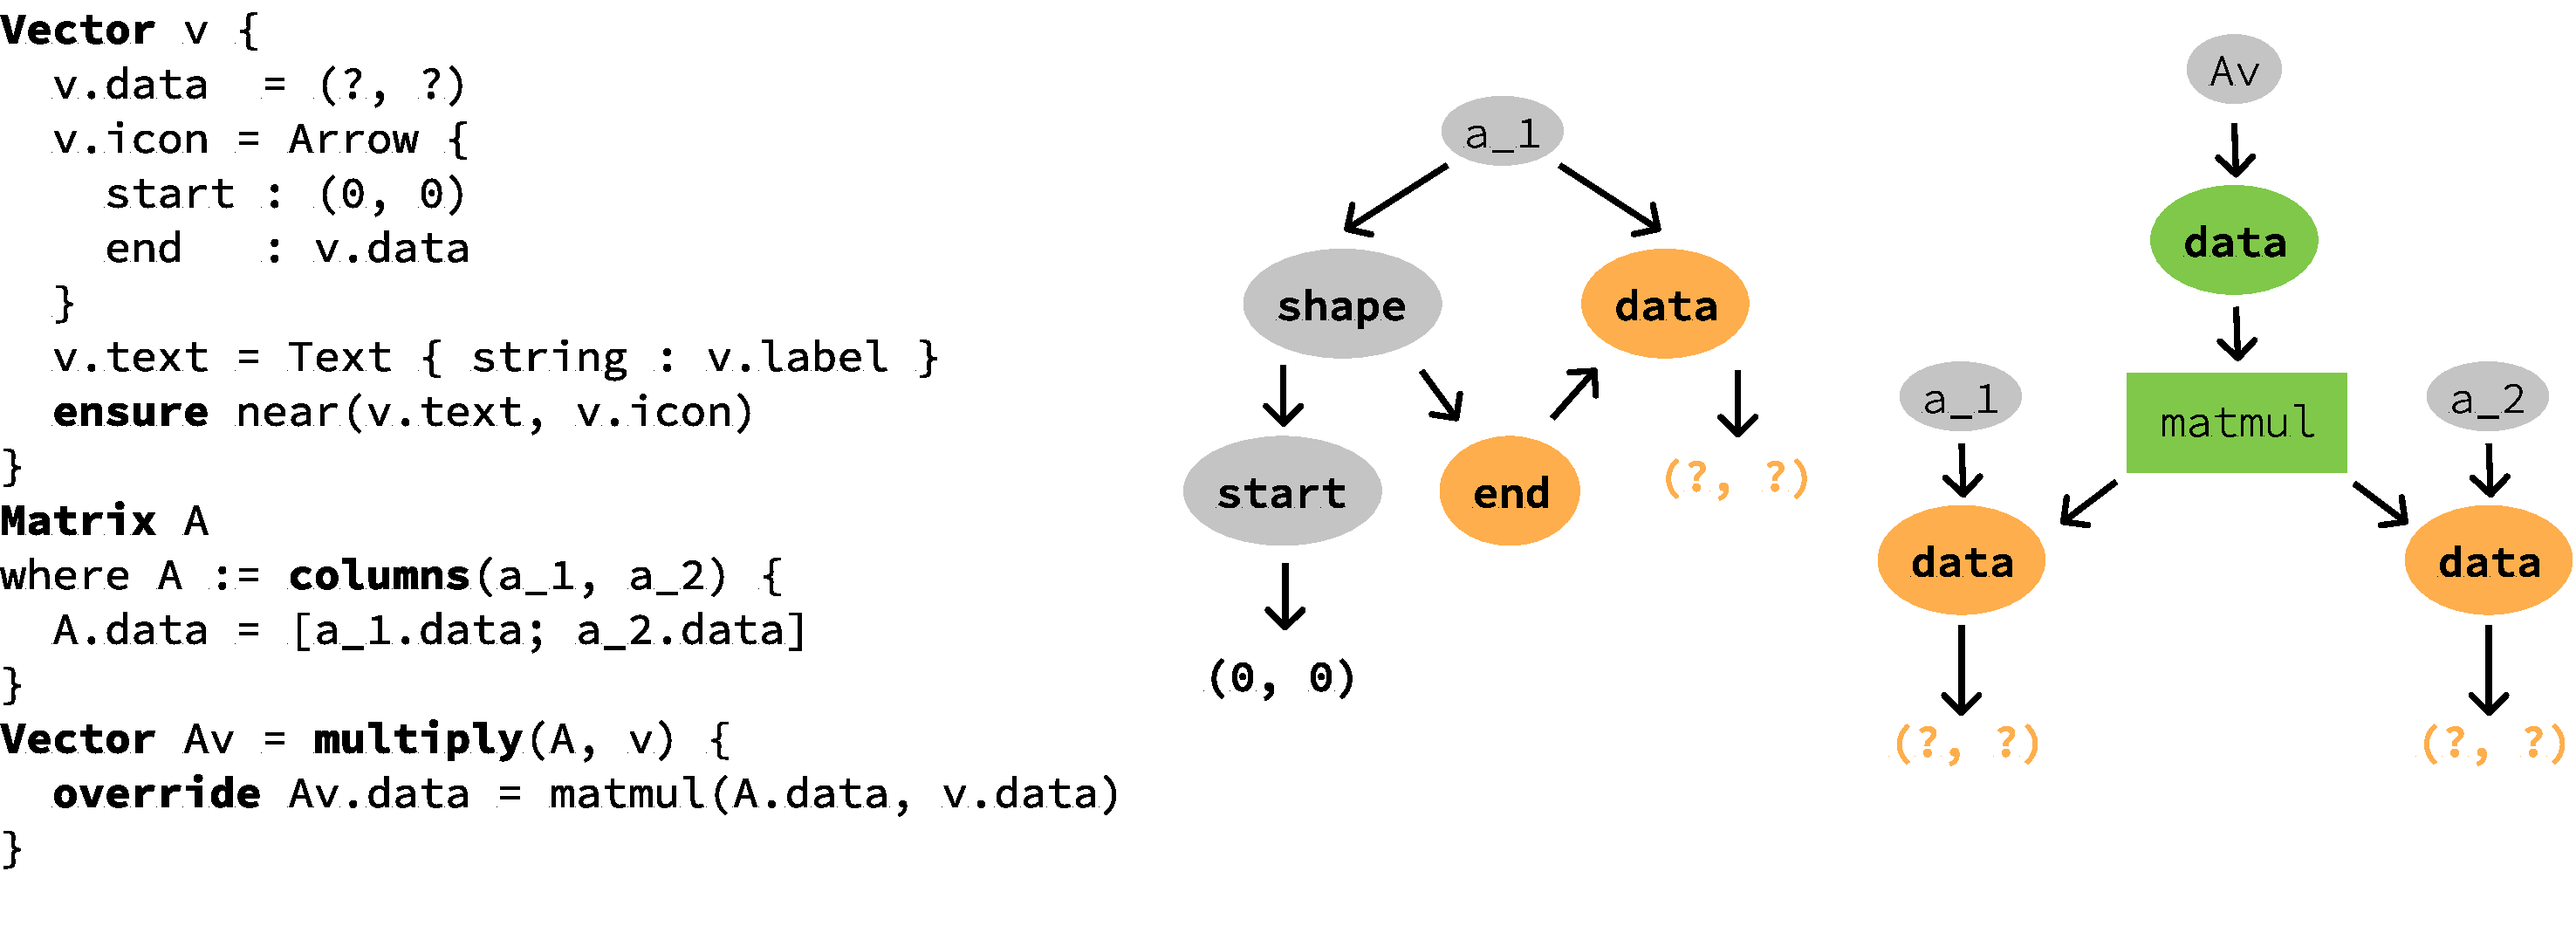
\includegraphics[width=\linewidth]{assets/chapter-4/eigen-comp-graph.pdf}
%     \vspace{-30pt}
%     \caption{\textbf{Left}: relevant blocks in the linear algebra \Style program for \cref{sec:ipenrose-example}. \textbf{Right}: computational graphs for \texttt{a\_1} and \texttt{Av}, where the \texttt{data} field for the former is optimized and that for the latter is computed.}
%     \label{fig:eigen-comp-graph}
% \end{figure}
% \vspace{10pt}

% Once exposed as draggable properties, the user can now change the values of positional DOFs by dragging shapes around. However, since their interaction is situated in an optimization problem, it's important to discuss how an optimizer influences this interaction and manipulates the rest of the diagram in a semantics-preserving way. In \cref{sec:ipenrose-example}, dragging \sty{a_1.icon.end} and \sty{a_2.icon.end} works as intended because they are independent from each other: they don't participate in the same constraints in the computational graph. However, this is not the right interaction for DOFs that participate in the same constraints, which is often the case. In this section, I give two example optimization strategies for supporting semantics-preserving drag.    
% \subsection{Follow the cursor}
% \label{sec:follow-the-cursor}

% \vspace{10pt}
% \begin{figure}[h]
%     \centering
%     \includegraphics[width=0.8\linewidth]{assets/chapter-4/drag-expected.pdf}
%     \caption{Dragging a subset, $B$, in a Venn diagram in an intuitive and semantics-preserving way, where $B$ is always under the cursor and $B \subset A$ is always held true.}
%     \label{fig:drag-expected}
% \end{figure}
% \vspace{10pt}

% Consider the example in \cref{fig:drag-expected}, which shows a simple Venn diagram of sets $A$ and $B$ where $B \subset A$. The underlying rule of this visual representation is that a subset is always visually contained in the superset. An interactive diagram should clearly reveal this rule by keeping this containment relationship true at all times. For instance, if a student drags $B$ to the right, the diagram should change such that $A$ still contains $B$. Importantly, the interaction should be natural, and also make the feedback very clear: as the student is dragging $B$, $B$ must stay under the cursor, and the rest of the diagram should incrementally move with $B$ to maintain the containment relationship.

% Unfortunately, when using the current \Penrose optimizer, dragging either $A$ or $B$  yields counterintuitive results: the optimizer changes arbitrary properties, including the manipulated ones. This is because it optimizes all DOFs simultaneously. In \cref{fig:drag-default}, it moves both $A$ and $B$ to satisfy the containment constraint.  This behavior adds noise to the feedback, and may confuse the student.

% \vspace{10pt}
% \begin{figure}[h]
%     \centering
%     \includegraphics[width=0.75\linewidth]{assets/chapter-4/drag-default.pdf}
%     \caption{Dragging a subset, $B$, in a Venn diagram in semantics-preserving but counterintuitive way, where $B \subset A$ held true but the shapes appear in random locations.}
%     \label{fig:drag-default}
% \end{figure}
% \vspace{10pt}

% To enable intuitive interactivity, the system can analyze the computational graph again to derive the right behavior. We can achieve this behavior by ``locking'' the DOFs, treating them as constants in the optimizer. Specifically, when a student manipulates DOFs or its aliases, the system locks these DOFs and optimizes the rest as usual. When the student interacts with an object (\ie, dragging to change \sty{x} and \sty{y} of a \sty{Circle}), the system yields the control to the student completely and locks the manipulated properties during optimization. The visual effect is that all other parts of the diagram ``follow'' the student interaction. 

% \subsection{Freeze the world}
% \label{sec:freeze-the-world}

% Locking the manipulated property is not the only way to maintain the visual semantics. Instead of limiting the optimizer, we could also limit the interaction so they see the effect of changing one or multiple shape properties under constraints. When the student interacts with a shape, the optimizer keeps all other properties locked and continuously uses the energy function to “guide” the student. The techniques involved are different from \cref{sec:follow-the-cursor}. In this case, the student is playing the role of the optimizer, \ie, changing DOFs, while the optimizer only sends feedback to make sure the interaction is semantic. The visual effect is a constrained interaction where the student can only make semantically-valid moves. 

% \vspace{10pt}
% \begin{figure}[h]
%     \centering
%     \includegraphics[width=0.75\linewidth]{assets/chapter-4/unit-circle-drag.pdf}
%     \caption{The behavior of dragging a point along the unit circle depends on the optimization strategy. \textbf{Left}: ``Follow the cursor'' shifts the entire diagram to follow the point and doesn't correspond to the mathematical semantics. \textbf{Right}: ``Freeze the world'' should be the correct optimization strategy, where the point only moves along the circle, and nothing else changes in the diagram.}
%     \label{fig:unit-circle-drag}
% \end{figure}
% \vspace{10pt}


% For instance, \cref{fig:unit-circle-drag} shows a diagram of the unit circle. A natural interaction is to drag the point along the unit circle to see how the values of trig functions change. In this case, the red line shows the value of $sin$. If the optimizer naively follows the cursor, \cref{fig:unit-circle-drag} (right) would be the result, where the rest of the diagram is translated to stay in a valid layout. Instead, it's much more desirable to ``freeze the world'' and constrain the student input within the feasible region—--along the unit circle (\cref{fig:unit-circle-drag} left).

% Together, these two strategies cover a wide range of drag behaviors that are traditionally difficult and time-consuming to implement. Note that these two strategies are not necessarily mutually exclusive. In fact, the system may have a set of default rules for or let the author specify the strategy on a per-DOF basis. For instance, an instructor might apply ``freeze the world'' to show students the valid positions of a component in a diagram, while applying ``follow the cursor'' to the rest of the components to show alternative layouts of the diagram. 


% \vspace{10pt}
% \noindent\textbf{Encoding optimization strategies.} If the author wants to control the optimization strategy, they will need an encoding to do so. Because \Style already has language constructs for matching on shapes, a \Style language extension may be suitable for specifying static strategies per shape, \eg, a shape should always follow the cursor when dragged. However, the current design of \Style may not be suitable for deciding strategies dynamically if needed, \eg, a shape follows the cursor in a certain region of the diagram, and freezes the world on the boundary. 
% \end{proposed}

% \section{Highlighting and annotation as feedback}
% \label{sec:highlight-and-annotate}

% \begin{proposed}

% As demonstrated in \cref{chp:edgeworth}, diagram understanding is a vital step towards representational fluency. A significant part of diagram understanding maps to learning the translational semantics of a diagram, \ie, which shape represents what math object. While \Edgeworth helps students practice the mapping between a particular visual representation and symbols, I propose to \textbf{provide on-demand, inter-representational feedback by utilizing the translational semantics of a \Penrose trio}. 

% \subsection{Inter-representational highlighting}

% Students' exposure to visual representations is often limited by traditional media like textbooks and in-person lectures. The mapping between symbolic and visual representations is often scarcely presented via prose, gesture, and carefully designed worked examples. Web-based materials show a much more pervasive use of on-demand highlighting to build up inter-representational connections. However, there’s also a non-trivial authoring burden to meticulously annotate the HTML document and the diagram with CSS classes:

% \vspace{10pt}
% \begin{figure}[h]
%     \centering
%     \includegraphics[width=\linewidth]{assets/chapter-4/euclid-highlight.pdf}
%     % \label{fig:euclid-highlight}
% \end{figure}
% \vspace{10pt}

% If an online textbook or website uses diagrams generated by \Penrose, the author may leverage the translational semantics to automatically provide on-demand highlights. For instance, suppose an author writes an visual explanation in markdown with interleaving \Substance symbols in the prose. The system can automatically generate diagrams by extracting the \Substance symbols and provide highlights for all subsequent references to the same symbols. Since \Penrose can generate alternative diagrams in the same visual presentations, the highlighting can also provide contrasting cases of a particular entity across diagram instances.

% \vspace{10pt}
% \begin{figure}[h]
%     \centering
%     \includegraphics[width=\linewidth]{assets/chapter-4/markup-highlight.pdf}
% \end{figure}
% \vspace{10pt}

% Building connections among multiple visual representations also improve learning~\cite{multipleReps}. Because a \Penrose trio is representationally salient, one can swap among alternative \Style programs to get diagrams that visualize the same symbols. Because the \Substance program stays the same, the same strategy also works for highlighting diagram parts across multiple visual representations.

% \vspace{10pt}
% \begin{figure}[h]
%     \centering
%     \includegraphics[width=0.9\linewidth]{assets/chapter-4/multirep-highlight.pdf}
% \end{figure}
% \vspace{10pt}

% \subsection{Documentation and program slices as tooltips} 

% \vspace{10pt}
% \begin{figure}[h]
%     \centering
%     \includegraphics[width=\linewidth]{assets/chapter-4/docs-tooltips.pdf}
% \end{figure}
% \vspace{10pt}

% In technical documents, symbols and acronyms are often defined once and used everywhere else. To help readers understand them, tools like ScholarPhi and Nota~\cite{scholarPhi, nota} use tooltips to aid readers. In real world publications, authors augment math equations for better readability, too. Diagrams use even more symbolism and can be hard to understand. We propose a lightweight markup language in the form of \Substance documentation for authoring simple \emph{diagram augmentation}. Similar to Idyll~\cite{idyll}, the markup language has a markdown-like syntax, but allows splices of \Substance variables and runtime values. In the frontend, we analyze the \Substance values in each snippet, and trace all related snippets based on variable references. For instance, the snippet about $Av$ refers to both $A$ and $v$, so they appear on the tooltip stack.

% The translational semantics also involve how \Domain, \Substance, and \Style programs relate to each other. Therefore, \Style and \Domain can also be valuable sources of feedback: the \Style program encodes the visual semantics, and the \Domain program captures the grammar of notations. A slice of a \Penrose trio traces the origin of a graphical primitive to the \Domain, \Substance, \Style programs. For instance, without any authoring burden, the system can display slices of the program trio based on object selection. Alternatively, the proposed markup language may be extended to \Domain and \Style, and the system can render inline documentations in all three languages.

% \vspace{10pt}
% \begin{figure}[h]
%     \centering
%     \includegraphics[width=0.75\linewidth]{assets/chapter-4/slices.pdf}
% \end{figure}
% \vspace{10pt}
% \end{proposed}

% \section{Evaluation}

% \begin{proposed}
% To evaluate the discussed interactive techniques, I plan to conduct comparative case studies between feature-full modern JavaScript libraries (e.g. D3.js) and \Penrose. Research questions for this study include:
% \begin{itemize}
%     \item Does the \Penrose-based system simply programming interactive diagrams?
%     \item Are the interactive features comparable to the hand-written examples? 
%     \item How expressive is our grammar of interactivity?
%     \item When does the approach break down?
% \end{itemize}

% In general, I expect that our system can cover common, important interactive features with significantly less manual effort. In the studies, I plan to collect both quantitative (\eg, lines-of-code, time taken) and qualitative data about authoring interactive diagrams using JS library versus our system. Currently, the candidate pool of examples include:

% \begin{itemize}
% \item Worked examples and explorable explanations:
%     \begin{itemize}
%         \item A Gentle Introduction to Graph Neural Networks: \url{https://distill.pub/2021/gnn-intro/}
%         \item Explained visually: \url{https://setosa.io/ev/}
%         \item Explorable explanations: \url{https://explorabl.es/}
%         \item Gallery of concept visualization: \url{https://conceptviz.github.io/}
%     \end{itemize}
% \item Online textbooks and curricula:
%     \begin{itemize}
%         \item Seeing theory: \url{https://seeing-theory.brown.edu/}
%         \item Immersive math: \url{http://immersivemath.com/ila/index.html}
%         \item Mathigon: \url{https://mathigon.org/}
%         \item Physically-based rendering: \url{https://pbr-book.org/}
%         \item Brilliant: \url{https://brilliant.org/}
%     \end{itemize}
% \end{itemize}
% \end{proposed}

% \section{Related work}

% \subsection{Grammars for interactivity}

% Pioneered by the grammar of graphics~\cite{grammarOfGraphics}, researchers in data visualization developed a rich set of tools based on an explicit encoding of the mapping from data to visual primitives~\cite{d3, vega, vegalite}. Notably, Vega-Lite~\cite{vegalite} is a grammar for interactive data visualization. One key to the Vega-Lite grammar is ``selection,'' because the underlying data doesn't change during interaction. In diagramming, this assumption is not always true. The basic building blocks are mostly ``manipulation'' of shapes in relation with the underlying representation. \citet{datavizCriticalReflection} give an extensive review of data visualization authoring tools, including those that support interactivity.

% In addition, the information/data visualization literature also contributed taxonomies and conceptual frameworks of interactivity. For instance, \citet{infovizInteractionFramework} propose 7 general categories of interactive techniques in information visualization: Select, Explore, Reconfigure, Encode, Abstract/Elaborate, Filter, and Connect. Similarly, \citet{interactiveDynamicsTaxonomy} describe a taxonomy of interactive dynamics for visual analysis, which was presented as a list of verbs, too. These frameworks and taxonomies are useful to build upon. Again, the high-level concepts involved for interactive diagrams can change significantly from them because of the differences between diagrams and data/information visualization~\cite{naturalDiagramming}, 

% \subsection{Constraint-based interactivity}

% In the HCI literature, there’s a long line of work on authoring interactive user interfaces using constraints. For instance, Garnet~\cite{garnet} and Amulet~\cite{amulet} use dataflow constraints to build highly interactive UIs. In these systems, the author declaratively specifies constraints on the relationship among graphical elements in terms of data dependencies (i.e. $D = f(l_1, l_2, \dots, l_n)$, and the interactivity is handled by a constraint solver at runtime. Thinglab~\cite{thinglab} supports simultaneous equations for building simulations. At its core, the \Penrose system is a combination of dataflow constraints (computations) and simultaneous equations (constraints and objectives). Therefore, many of the techniques from this line of work may apply to supporting interactivity in \Penrose, such as efficient incremental constraint solving~\cite{deltablue}.


% \chapter{\Edgeworth project plan}

% To address the committee feedback from the thesis proposal presentation, this appendix to the proposal document elaborates on \cref{chp:edgeworth}. This elaboration comes in acknowledgment that the committee sees the goals in \cref{chp:ipenrose} as optional.  In this appendix, I summarize the proposed elaboration on \cref{chp:edgeworth}, describe the research hypotheses, and outline the evaluation plan for validating them. The intention of this appendix is to specify all of the required work in the dissertation.

% In the proposal document, \cref{chp:edgeworth} describes the following completed work on \Edgeworth:

% \begin{itemize}
%     \item Formative interviews with 6 educational content authors
%     \item Design and implementation of mutation operators in the \Edgeworth mutator
%     \item A prototype of the \Edgeworth mutator with a configuration-based workflow
%     \item Preliminary evaluation of the prototype by re-creating problems in a geometry textbook
% \end{itemize}